\noindent\textcolor{stewartblue}{\textbf{VÍ DỤ 3}}\hspace{0.8em}Tìm $\displaystyle\lim_{x \to 0} \left( x^3 + \frac{\cos 5x}{10{,}000} \right)$.

\vspace{0.45em}
\noindent\textcolor{stewartblue}{\textbf{LỜI GIẢI}}\hspace{0.8em}Như trước đây, chúng ta lập một bảng giá trị. Từ bảng thứ nhất, có vẻ như giới hạn có thể bằng không.

\begin{center}
\renewcommand{\arraystretch}{1.2}
\small
\begin{tabular}[t]{|l|c|}
\hline
\rowcolor{tableheader}
\multicolumn{1}{|c|}{$x$} & $x^3 + \dfrac{\cos 5x}{10{,}000}$ \\
\hline
1    & 1.000028 \\
0.5  & 0.124920 \\
0.1  & 0.001088 \\
0.05 & 0.000222 \\
0.01 & 0.000101 \\
\hline
\end{tabular}%
\hspace{1.2cm}%
\begin{tabular}[t]{|l|c|}
\hline
\rowcolor{tableheader}
\multicolumn{1}{|c|}{$x$} & $x^3 + \dfrac{\cos 5x}{10{,}000}$ \\
\hline
0.005 & 0.00010009 \\
0.001 & 0.00010000 \\
\hline
\end{tabular}
\end{center}

\vspace{0.2em}
\noindent
Nhưng nếu kiên trì với các giá trị nhỏ hơn của $x$, bảng thứ hai cho thấy rằng giới hạn nhiều khả năng là 0.0001. Trong Mục 2.5, chúng ta sẽ có thể chỉ ra rằng $\lim_{x \to 0} \cos 5x = 1$ và từ đó suy ra rằng
\begin{equation*}
\lim_{x \to 0} \left( x^3 + \frac{\cos 5x}{10{,}000} \right) = \frac{1}{10{,}000} = 0.0001 \tag*{\textcolor{stewartblue}{\blacksquare}}
\end{equation*}

\vspace{0.8em}
\noindent{\color{stewartblue}\rule{1.15ex}{1.15ex}}\hspace{0.55em}{\large\textbf{Giới hạn một phía}}

\vspace{0.5em}
\noindent
\marginnote{%
  \centering
  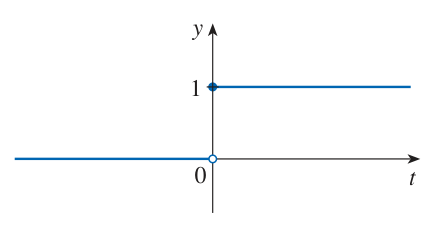
\includegraphics[width=\marginparwidth]{images/p0121_fig1.png}\\[4pt]
  {\small\textbf{\color{stewartblue}HÌNH 5}\\[1pt]
  Hàm Heaviside}%
}[-0.3cm]%
Hàm Heaviside $H$ được định nghĩa bởi
\[
H(t) = \begin{cases}
0 & \text{nếu } t < 0 \\
1 & \text{nếu } t \ge 0
\end{cases}
\]
(Hàm số này được đặt theo tên của kỹ sư điện Oliver Heaviside [1850--1925] và có thể được dùng để mô tả một dòng điện được bật tại thời điểm $t = 0$.) Đồ thị của nó được thể hiện trong Hình 5.

\vspace{0.45em}
\noindent
Không có một số duy nhất nào mà $H(t)$ tiến tới khi $t$ tiến dần đến 0, do đó $\lim_{t \to 0} H(t)$ không tồn tại. Tuy nhiên, khi $t$ tiến dần đến 0 từ bên trái, $H(t)$ tiến tới 0. Khi $t$ tiến dần đến 0 từ bên phải, $H(t)$ tiến tới 1. Ta biểu diễn điều này bằng ký hiệu
\[
\lim_{t \to 0^-} H(t) = 0 \qquad \text{và} \qquad \lim_{t \to 0^+} H(t) = 1
\]
và ta gọi đây là các \emph{giới hạn một phía}. Ký hiệu $t \to 0^-$ chỉ ra rằng chúng ta chỉ xét các giá trị của $t$ nhỏ hơn 0. Tương tự, $t \to 0^+$ chỉ ra rằng chúng ta chỉ xét các giá trị của $t$ lớn hơn 0.

\vspace{0.6em}
\begin{tcolorbox}[
  colback=white,
  colframe=stewartred,
  boxrule=1.1pt,
  sharp corners,
  boxsep=0pt,
  left=8pt,
  right=8pt,
  top=7pt,
  bottom=7pt
]
\noindent
{\setlength{\fboxrule}{1pt}\setlength{\fboxsep}{2.5pt}\fbox{\color{stewartred}\textbf{2}}}\hspace{0.5em}{\textbf{\color{stewartred}Định nghĩa trực quan về giới hạn một phía}}\hspace{1.5em}Ta viết
\vspace{-0.2em}
\[
\lim_{x \to a^-} f(x) = L
\]
\vspace{-0.3em}
\noindent
và nói rằng \textbf{giới hạn bên trái} của $f(x)$ khi $x$ tiến tới $a$ [hoặc giới hạn của $f(x)$ khi $x$ tiến tới $a$ \emph{từ bên trái}] bằng $L$ nếu ta có thể làm cho các giá trị của $f(x)$ gần $L$ tùy ý bằng cách giới hạn $x$ đủ gần $a$ \emph{với $x$ nhỏ hơn $a$}.

\vspace{0.5em}
\noindent\hspace{1.5em}Ta viết
\vspace{-0.2em}
\[
\lim_{x \to a^+} f(x) = L
\]
\vspace{-0.3em}
\noindent
và nói rằng \textbf{giới hạn bên phải} của $f(x)$ khi $x$ tiến tới $a$ [hoặc giới hạn của $f(x)$ khi $x$ tiến tới $a$ \emph{từ bên phải}] bằng $L$ nếu ta có thể làm cho các giá trị của $f(x)$ gần $L$ tùy ý bằng cách giới hạn $x$ đủ gần $a$ \emph{với $x$ lớn hơn $a$}.
\end{tcolorbox}
